\subsection{Training cohorts and representative selection}
\label{sec:cohorts}
The comparison contains three trainable tree families: axis-aligned cuts with
linear leaves, oblique cuts with constant leaves, and oblique cuts with linear
leaves. Their common reference is the 100-tree axis-aligned, constant-leaf
boosted ensemble. Table~\ref{tab:comparison}, placed last in the document,
contains the ten selected configurations. Within each family we retain its
highest eligible working-point efficiency and two smaller representatives,
rather than the three largest efficiencies irrespective of size. This is a
compact selection of operating points, not an exhaustive Pareto frontier.

The axis/linear cohort uses $T\in\{1,3\}$ and $D\in\{3,4\}$, giving four
layouts, with $\lambda_s=0$ and $\lambda_\ell=10^{-5}$. All four source runs
converged. Each terminal source then supplied its exact leaf support for an
unpenalized leaf-only refit, with cuts held fixed. Three refits converged; the
three-tree depth-four refit detected logistic separation and was held. Its
regularized source remains eligible. For each layout we select the best saved
working-point checkpoint from eligible source/refit stages. The selected
three-tree depth-three model has 274 learned nonzero scalars and 53.83\%
efficiency; the single depth-four tree has 228 and 54.74\%. We therefore omit
the former from the three representatives, although its AUC is slightly
higher. This decision follows the stated low-background objective. All four
layouts are reported in Appendix~\ref{app:axis}.

The oblique/constant cohort scans $T\in\{1,3,5\}$, $D\in\{2,3,4\}$ and
$\lambda_s\in\{0,10^{-7},10^{-5}\}$: all 27 source configurations converged.
The nominal leaf penalty has no effect because constant leaves have no feature
weights. Selecting the best eligible penalty/checkpoint for each layout gives
the three depth-four representatives with one, three and five trees. The full
nine-layout summary is in Appendix~\ref{app:constant}.

For oblique/linear forests, the architecture study varies tree count, depth
and separate cut/leaf penalties, while a further support study applies
\SFR{}. At the comparison snapshot, 57 of 58 architecture configurations had
converged; unfinished sources are excluded. The highest eligible efficiency
is 57.73\% from five depth-four trees, trained with
$\lambda_s=\lambda_\ell=10^{-5}$ and selected at epoch 21 of its converged
source run. The other representatives are a completed leaf-only refit with
837 nonzeros at 57.12\%, and the 418-nonzero Compact refit at 56.20\%.
The former's subsequent full refit was held and is excluded. Compact refit's
full source stage converged at epoch 15; its selected snapshot is epoch 8.
The support study and training chain are given in Appendix~\ref{app:support}.

Convergence is required of the source stage, not necessarily of an earlier
validation-selected snapshot. Different families and representatives have
different penalty and refitting histories. The table compares implementation
candidates, rather than isolating a causal effect of leaf type at identical
support, initialization trajectory or hyperparameter budget.

\begin{implementation}
\textbf{Pinned comparison.}
\file{scripts/compare_ten_models.py} selects and checks the ten entries;
\file{docs/ten_model_comparison_v1/validation.json} records their metrics,
source hashes, checkpoint hashes, layouts and measured timing.
The frozen document input is \code{paper/sources/ten_model_comparison.json}.
\file{scripts/check_comparison_working_points.py} checks both the scalar C++
and portable NumPy calibrations on all validation events; the report is
\file{docs/ten_model_comparison_v1/working_point_checks.json}.
The newest oblique/linear winner is case 50 of
\file{configs/tao_hyper_scan_v1.json}, with its exact worker policy in
\file{configs/hyper_scan_v1/case_50.json}. The axis cohort is pinned by
\file{configs/axis_linear_v1.json}; its four regularized and refit policies
are in \code{configs/axis_linear_v1/}. The axis refits run only the existing
\code{leaf_only} stage, preserving axis cuts and the selected exact-zero leaf
mask. The old 57.12\% result is now a smaller representative, not the current
oblique/linear performance winner. The historical v3 default remains Compact
refit; no firmware resource winner has been selected.
\end{implementation}

\subsection{Validation performance and parameter use}
\label{sec:family-results}
Figure~\ref{fig:families} compares the selected ROCs; Fig.~\ref{fig:family-cost}
shows their working points against scalar and multiplication budgets.
The XGBoost reference reaches 55.48\% signal efficiency at 1\% background.
The five-tree oblique/linear forest reaches 57.73\% with 1275 nonzero scalars.
At almost the same scalar count, five oblique/constant trees use 1250 and
reach 55.40\%. Their respective AUCs are 0.93090 and 0.92610, compared with
0.92056 for XGBoost. These are observed validation differences; model
selection and training variation preclude an independent accuracy claim.

\begin{figure}[htbp]\centering
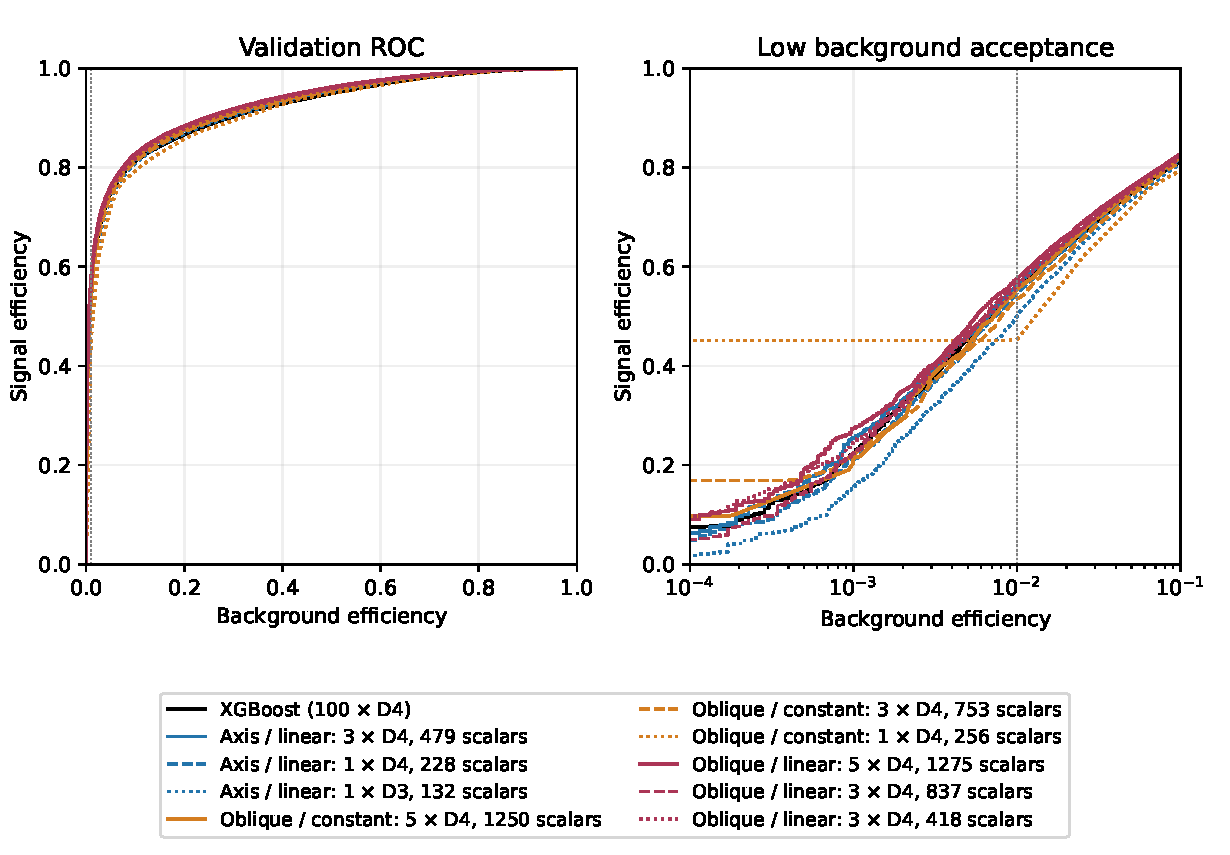
\includegraphics[width=\textwidth]{figures/family_roc.pdf}
\caption{The ten selected configurations on the same validation partition.
Colors identify families; line styles distinguish their representatives.
The low-background panel resolves the primary working point.
Numbers in the legend are learned nonzero scalar counts, with the axis-cut
storage convention defined in the text.}
\label{fig:families}
\end{figure}

Linear leaf functions can compensate for a smaller or sparser partition.
Compact refit reaches 56.20\% with 418 nonzeros (379 after input-independent branch pruning), approximately three times
fewer than the 1250-coefficient constant-leaf winner. This comparison includes
both cut and leaf coefficients: a richer leaf increases its own arithmetic,
but can reduce the overall number of retained cuts and weights. Conversely,
axis-aligned routing can remain competitive when the leaves are expressive.
A single axis-aligned depth-four tree reaches 54.74\% using 228 learned
nonzero scalars and 15 feature choices/direction bits. Three such trees reach
56.32\% using 479 scalars and 45 discrete cut choices.

The distinction between interpolation and a realizable threshold matters most
for coarse constant-leaf scores. The constant-leaf winner's interpolated
55.40\% becomes 54.75\% at a strict threshold respecting the 525-background
event budget. The selected linear-leaf entries retain their displayed
working-point efficiencies under the strict-threshold convention. A high AUC
alone does not establish a better low-background selection. A strict threshold
is tied to its numerical evaluator: changing even binary64 reduction order can
move an event at the cut, so the working point must be checked again after a
change of arithmetic, not only after quantization.

\begin{figure}[htbp]\centering
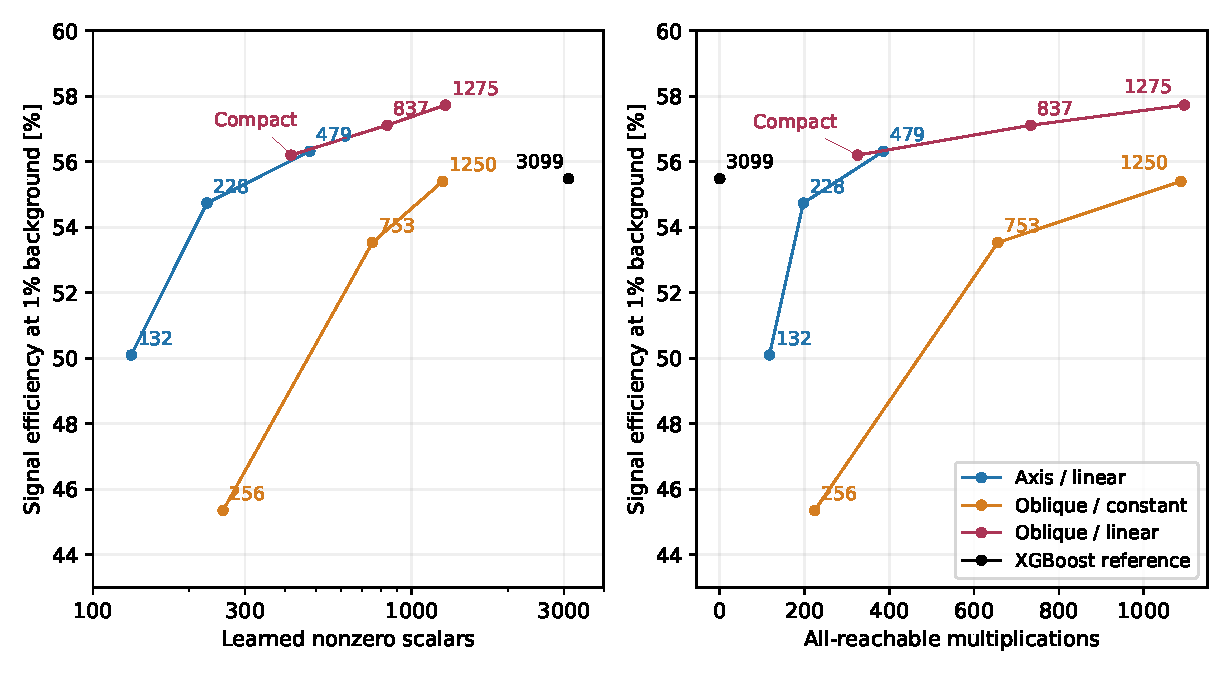
\includegraphics[width=\textwidth]{figures/family_tradeoff.pdf}
\caption{Representative validation operating points versus learned nonzero
scalars (left) and all-reachable multiplications after exact-zero/unit-factor
elimination (right). Lines only connect the selected representatives.
Labels identify scalar counts; Compact denotes the 418-coefficient refit.
Feature indices, direction bits, comparisons and additions are separate costs.
XGBoost uses no general multiplications here, but still performs tree decisions
and score aggregation.}
\label{fig:family-cost}
\end{figure}

\subsection{Matched CPU evaluation and arithmetic workload}
\label{sec:cost}
The C++ column in Table~\ref{tab:comparison} uses one common sparse path-traversal
reference for all ten models. Inputs and coefficients are binary64, with
XGBoost inputs rounded to binary32 before traversal to preserve its native
feature semantics. Exact-zero and unit-factor operations are eliminated;
axis cuts use direct comparisons. All node and coefficient structures are
loaded before timing. With one thread, one untimed warmup and nine timed
repeats of the full 132,800-event batch, we report median wall time divided
by event count. Parsing, preprocessing, allocation, input conversion and file
I/O are excluded. The measurement host is a KVM guest reporting Intel Xeon
Gold 6138 processors with a nominal 2.00 GHz clock; no fixed-frequency control
is assumed. Compilation uses GCC 12.3.1, C++17, optimization level 3 and disabled
fused multiply-add contraction. The results measure bulk throughput, not
single-event latency.

The axis three-tree depth-four model takes 0.101 microseconds per event,
compared with 0.167 for Compact refit, 0.412 for the five-tree oblique/linear
winner and 0.965 for the five-tree constant-leaf winner. The common reference
takes 3.675 microseconds for XGBoost. Separately, the optimized native XGBoost
library takes 1.478 microseconds per event on the same host and batch,
including probability output. Thus the common kernel is a controlled
reference, not the best achievable software implementation of every model.
Differences from earlier NumPy and C++ prototype timings must not be read as
changes in the algorithms' intrinsic cost.

The choice of hardware schedule changes the relevant arithmetic comparison.
Axis three-tree depth-four routing requires no general multiplications, and
its selected-path bound is 35 leaf products, versus 78 total products for
Compact refit. Computing all reachable affine functions instead requires 386
products for the axis model and 325 for Compact refit. Their path comparison
bounds are both 12. The axis model therefore has fewer sequential-path
products, but more scalars (479 versus 418), more all-node products and
additional discrete cut choices. Neither point uniformly dominates the other.
XGBoost has zero general products because the learning rate is absorbed into
its leaf values, yet has up to 400 path comparisons and 1499 internal decisions
in an all-node evaluation. Multiplication count alone cannot rank all designs.

\begin{implementation}
\textbf{One timing kernel and independent checks.}
\file{fpga/comparison/benchmark.cc} implements the shared sparse reference.
\file{scripts/run_ten_model_comparison.sh} uses the pinned EL9/CMSSW environment;
\file{scripts/compare_ten_models.py} prepares canonical models and validates
predictions and every leaf assignment before recording results (16.6 million assignments across
the ten validation predictions). The host was
\code{clip-c2-48.cbe.vbc.ac.at}, with GCC 12.3.1,
\code{-O3 -std=c++17 -ffp-contract=off}. All leaf assignments match exactly on
validation. The largest XGBoost margin difference from native inference is
$2.89\times10^{-6}$; each TAO margin differs by less than $10^{-9}$.
\code{operations} counts nonzero, non-unit feature factors after constant-route
pruning. Older \code{sparsity_profile} counts retain unit products and are
therefore slightly larger; the final table uses the new convention consistently.
\file{paper/build_comparison_assets.py} regenerates the table from the frozen
report; \code{--plot} additionally needs archived validation scores on CLIP.
\end{implementation}
